
\begin{figure}
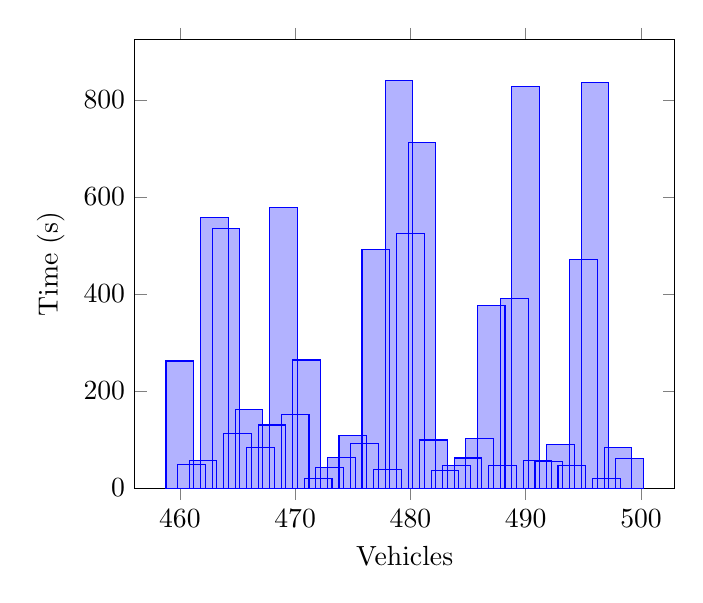
\begin{tikzpicture}
\begin{axis}[
legend style={anchor=west},
xlabel=Vehicles,
ylabel=Time (s),
ymin=0,
ybar,
]
\addplot coordinates {
(470, 151)
(496, 835)
(484, 46)
(474, 63)
(493, 89)
(479, 840)
(467, 83)
(491, 57)
(462, 57)
(492, 54)
(477, 492)
(468, 130)
(494, 47)
(498, 83)
(488, 46)
(495, 472)
(469, 579)
(471, 264)
(478, 39)
(482, 99)
(487, 376)
(460, 262)
(475, 109)
(473, 43)
(466, 162)
(481, 713)
(497, 20)
(465, 113)
(463, 557)
(486, 103)
(490, 828)
(476, 92)
(461, 49)
(499, 61)
(489, 390)
(483, 36)
(472, 20)
(464, 535)
(485, 62)
(480, 524)
};

\end{axis}
\end{tikzpicture}
\label{tik:time:0:79}
\caption{0 percent diving with GSC on route $79$}
\end{figure}
